\documentclass[11pt]{article}
\usepackage[utf8]{inputenc}
\usepackage[czech]{babel}
\usepackage[left=2cm,text={17cm, 24cm},top=3cm,a4paper]{geometry}
\usepackage{times}
\usepackage{csquotes}
\usepackage{graphics}
\usepackage{float}
\usepackage{multirow}
\usepackage{boldline}

\begin{document}

\begin{titlepage}
\begin{center}

\Huge\textsc{Fakulta informačních technologií\\
Vysoké učení technické v Brně}\\
\vspace{\stretch{0.382}}
\LARGE
\textbf{Překladač jazyka IFJ21\,-\,Projektová dokumentace}\\
Tým 004\,-\,varianta II.
\vspace{\stretch{0.100}}

\begin{table}[ht]
    \centering
    \begin{tabular}{l l l}
        \textbf{Vojtěch Eichler} & \textbf{xeichl01} & \textbf{25\,\%}\\
        Adam Zvara & xzvara01 & 25\,\%\\
        Václav Korvas & xkorva03 & 25\,\%\\
        Tomáš Matuš & xmatus37 & 25\,\%
    \end{tabular}
\end{table}
\vspace{\stretch{0.518}}

\Large
2021
\end{center}
\end{titlepage}

\section{Úvod}
Cílem tohoto projektu bylo vytvořit překladač, který přeloží zadaný jazyk IFJ21 do cílového mezijazyka \mbox{IFJCode2021.}
Jazyk IFJ21 je staticky typovaný a~imperativní jazyk. Jedná se o podmožinu jazyka Teal.
Překladač je napsaný v jazyce C.

\section{Implementace}
Překladač je sestaven ze 3 hlavních částí a to scanner, parser a generátor kódu.
Scanner provádí lexikální analýzu a načítání vstupního kódu, parser pak provádí syntaktickou a sémantickou analýzu.

\subsection{Lexikální analýza}
Lexikální analýza je implementována v souborech scanner.c a scanner.h. Hlavní funkce lexikálního analyzátoru je funkce \texttt{get\_token}, 
která postupně čte znak po znaku ze stdin. Tyto znaky poté převádní na strukturu \texttt{token\_t}. Tato struktura obsahuje atribut a typ tokenu. 
Jako typ tokenu může být identifikátor, řetězec, celé nebo desetinné číslo, EOF, aritmetické a porovnávací operátory nebo jiné znaky povolené v jazyce IFJ21. 
Atribut mají pouze tokeny typu řetězec, identifikátor, klíčové slovo nebo čísla. Zda-li se jedná o klíčové slovo nebo identifikátor
se stará pomocná funkce \texttt{check\_keyword}, která porovná danný řetězec se všemi klíčovými slovami, pokud se s žádným z nich neshoduje nastaví jako typ
tokenu identifikátor. Funkce \texttt{get\_token} pak také využívá řadu dalších pomocných funkcí například pro převod řetězce na číslo.

Lexikální analyzátor byl implementován na základě námi vytvořeného deterministického konečného automatu (DKA).
Tento DKA je implementován jako jeden nekonečně se opakující switch, kde jednotlivé přípády case reprezentují jednotlivé stavy tohoto automatu.
Pokud se automat dostane do jednoho z koncových stavů, tak se funkce ukončí a vrátí odpovídající token. Pokud ovšem
automat skončí v nekoncovém stavu nebo je načten znak, který není povolen v jazyce IFJ21, tak nastává lexikální chyba a funkce je ukončena s návratovým kódem 1.

Escape sekvence jsou řešeny za pomoci pole, do kterého se postupně ukládají znaky, které mohou být v rozsahu 0-9. Toto decimalní číslo jehož maximální
hodnota je 255, je poté převedeno na korespondující ASCII hodnotu. 

\subsection{Syntaktická analýza}
Syntaktická analýza je implementována metodou rekurzivního sestupu. Překlad zdrojového kódu začíná zavolaním funkce 
\texttt{parse} z funkce main ve zdrojovém souboru \texttt{main.c}. Následuje inicializace tokenu, do kterého lexikální analyzátor 
zapisuje hodnoty, globální tabulky symbolů, paměti pro postupné ukládání generovaných instrukcí a také se nainicializuje pomocná struktura. 

Během implementace jsme postupně zjišťovali,
že bychom pro generování a sémentickou kontrolu potřebovali držet v paměti různé hodnoty jako například počty parametrů u volání funkce,
 ukazatel na funkci do globální tabulky symbolů a několik dalších hodnot. Z tohoto důvodu jsme si vytvořili pomocnou strukturu
 \texttt{parser\_helper} a funkce nad ní, implementovanou v souboru \texttt{parser\_helper.c}.

 Z funkce \texttt{parse} se 
 syntaktický analyzátor postupně rekurzivně zanořuje podle sekvence tokenů, které získavá od lexikálního analyzátoru. Po celou 
 dobu běhu se v globální proměnné \texttt{ret} udržuje aktuální stav a pokud analyzátor objeví chybu, nebo nastane interní chyba, 
 tato proměnná se nastaví na nenulovou hodnotu a začne vynořování z rekurze. 

 Jedna z největších výzev byla absence ukončovacího 
 znaku za příkazem, nebo pevně stanovené pravidla odsazování, což zkomplikovalo práci s načtenými tokeny. Proto analyzátor pracuje 
 s proměnnou \texttt{backup\_token}, která kromě role dočasného držení tokenu, plní roli při rozhodování, zda je nutné načítat 
 další token, nebo je potřeba pracovat s tokenem který už má načtený. Tímto způsobem jsme řešili situaci, kdy je při 
 vyhodnocování výrazů nevyhnutelně načten jeden token za koncem výrazu, jinak totiž nejsme schopní určit konec výrazu. 
 
 Syntaktická analýza pracuje se dvěma typy tabulky symbolů. První z nich je globální tabulka symbolů, do které jsou na začátku 
 syntaktické analýzy uloženy vestavěné funkce a postupně během překladu i uživatelem definované funkce. Druhý typ tabulky je lokální 
 tabulka symbolů, na začátku funkce se vytvoří první lokální tabulka a při dalším zanoření do cyklu, nebo v těle podmínky se vytvoří 
 další, která se pomocí ukazatele napojí na ostatní lokální tabulky. Vznikne tak jednostranně vázaný seznam, na jehož začátku se nachází 
 nejvíce zanořená tabulka a končí tabulkou vytvořenou při vstupu do těla funkce. Průchodem seznamem lokálních tabulek jsme tak 
 schopni kontrolovat zda a případně v jakém bloku platnosti jsou proměnné definované. Obě tabulky jsou naimplementované v souboru
 \texttt{symtable.c}.

\subsubsection{Syntaktická analýza výrazů}

\subsection{Sémantická analýza}

\subsection{Generování kódu}

\section{Práce v týmu}

\subsection{Rozdělení práce}

\begin{table}[ht]
    \centering
    \begin{tabular}{|l|l|}
        \hline
        \textbf{Člen týmu} & \textbf{Přidělená práce} \\\hline
        Vojtěch Eichler & Vedoucí týmu, syntaktická analýza, sémantická analýza, testování \\
        Adam Zvara & Sémantická analýza, generování kódu, testování \\
        Václav Korvas & Lexikální analýza, testování \\
        Tomáš Matuš & Precedenční analýza výrazů, sémantická analýza, dokumentace \\\hline
    \end{tabular}
    \label{tabulka_rozdeleni_prace}
    \caption{Rozdělení práce v týmu}
\end{table}

\subsection{Komunikace}
Našim hlavním komunikačním nástrojem byl Discord.
Dále jsme se osobně setkávali na předem dohodnutých schůzkách ve studovnách a nebo se bavili během přestávek mezi přednáškami.

\subsection{Verzovací systém}
Pro verzování jsme používali nástroj \texttt{git} a pro vzdálené sdílení repozitáře jsme využili \texttt{GitHub}.

\section{Diagram konečného automatu}
\begin{figure}[H]
    \centering
    \vspace{0.1cm}
    \scalebox{0.5}{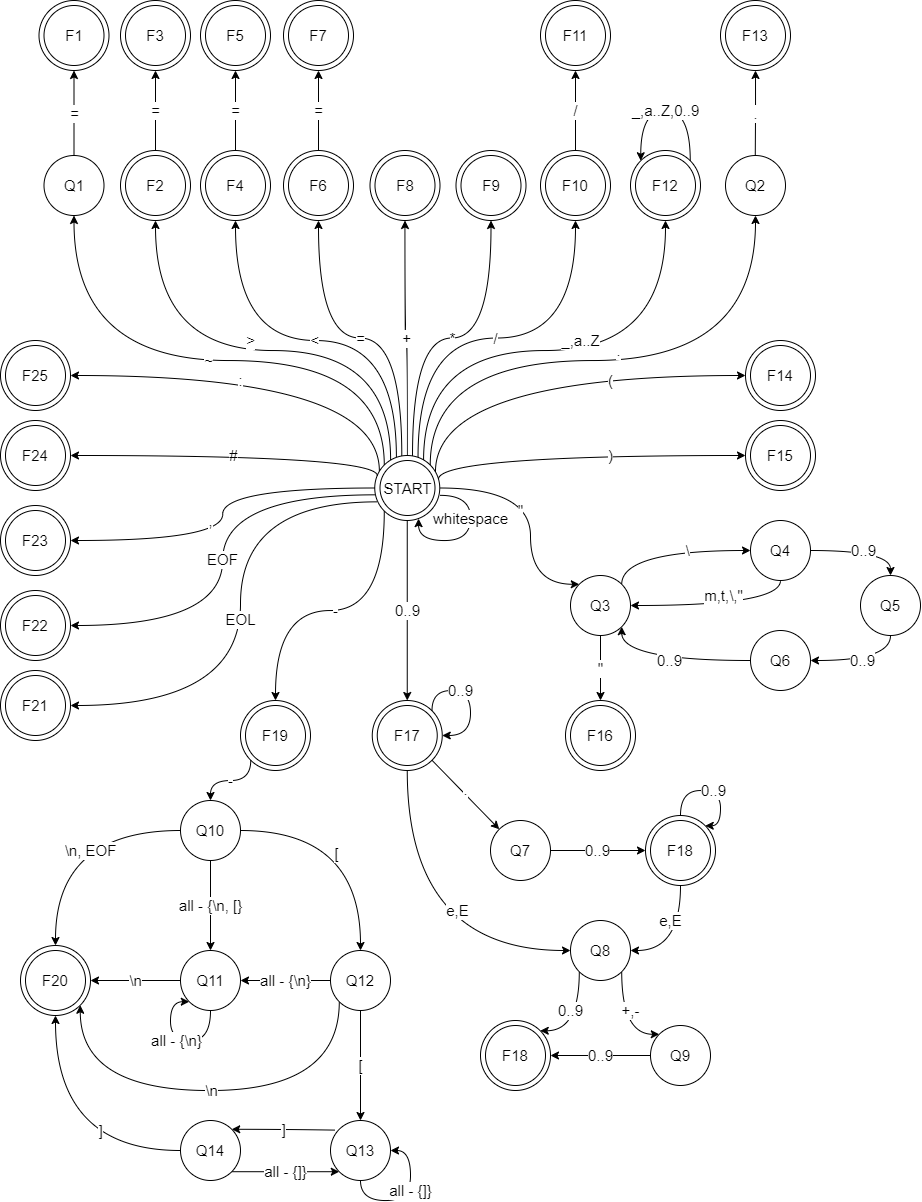
\includegraphics{doc/img/FSM.png}}
    \caption{Diagram konečného automatu specifikující lexikální analyzátor}
    \label{figure:fsm_img}
\end{figure}

\begin{table}[]
    \centering
    \begin{tabular}{|ll ll ll|}
        \hline
        F1 & \texttt{NOT\_EQUAL} & F14 & \texttt{LEFT\_BRACKET} & Q2 & \texttt{CONCAT\_START} \\
        F2 & \texttt{GREATER\_THAN} & F15 & \texttt{RIGHT\_BRACKET} & Q3 & \texttt{STRING\_START} \\
        F3 & \texttt{GREATER\_THAN\_EQUAL} & F16 & \texttt{STRING\_LITERAL} & Q4 & \texttt{STRING\_ESCAPE} \\
        F4 & \texttt{LESSER\_THAN} & F17 & \texttt{INTEGER} & Q5 & \texttt{STRING\_ESCAPE\_HEXADEC\_1} \\
        F5 & \texttt{LESSER\_THAN\_EQUAL} & F18 & \texttt{NUMBER} & Q6 & \texttt{STRING\_ESCAPE\_HEXADEC\_2} \\
        F6 & \texttt{ASSIGN} & F19 & \texttt{MINUS} & Q7 & \texttt{NUMBER\_START\_DOT} \\
        F7 & \texttt{IS\_EQUAL} & F20 & \texttt{COMMENT} & Q8 & \texttt{NUMBER\_E} \\
        F8 & \texttt{PLUS} & F21 & \texttt{EOL} & Q9 & \texttt{NUMBER\_E\_PLUS\_MINUS}\\
        F9 & \texttt{MUL} & F22 & \texttt{EOF} & Q10 & \texttt{COMMENT\_START} \\
        F10 & \texttt{DIV} & F23 & \texttt{COMMA} & Q11 & \texttt{COMMENT\_SKIP} \\
        F11 & \texttt{INT\_DIV} & F24 & \texttt{STRING\_LENGTH} & Q12 & \texttt{COMMENT\_BLOCK\_START} \\
        F12 & \texttt{ID} & F25 & \texttt{COMMA} & Q13 & \texttt{COMMENT\_BLOCK} \\
        F13 & \texttt{CONCAT} & Q1 & \texttt{NOT\_EQUAL\_START} & Q14 & \texttt{COMMENT\_BLOCK\_STOP} \\
        \hline
    \end{tabular}
    \caption{Legenda konečného automatu pro lexikální analýzu}
    \label{tab:FSM legenda}
\end{table}

\section{LL\,-\,gramatika}

\section{LL\,-\,tabulka}

\section{Precedenční taulka}
\begin{table}[h]
    \catcode`\-=12
    \centering
    \newcolumntype{?}{!{\vrule width 1pt}}
    \begin{tabular}{?c?c|c|c|c|c|c|c|c|c|c?}
        \hlineB{3}
        \multicolumn{11}{?c?}{\textbf{Načtený token}} \\\hlineB{3}
        \parbox[t]{2mm}{\multirow{10}{*}{\rotatebox{90}{\textbf{Vrchol stacku}}}}
        &&\# & * / // & + - & .. & r & ( & ) & id & \$                       \\\cline{2-11}
        &\#      & $-$ & $>$ & $>$ & $-$ & $>$ & $<$ & $-$ & $<$ & $>$       \\\cline{2-11}
        &* / //  & $<$ & $>$ & $>$ & $-$ & $>$ & $<$ & $>$ & $<$ & $>$       \\\cline{2-11}
        &+ -     & $<$ & $<$ & $>$ & $-$ & $>$ & $<$ & $>$ & $<$ & $>$       \\\cline{2-11}
        &..      & $-$ & $-$ & $-$ & $<$ & $>$ & $<$ & $>$ & $<$ & $>$       \\\cline{2-11}
        &r       & $<$ & $<$ & $<$ & $<$ & $-$ & $<$ & $>$ & $<$ & $>$       \\\cline{2-11}
        &(       & $<$ & $<$ & $<$ & $<$ & $<$ & $<$ & $=$ & $<$ & $-$       \\\cline{2-11}
        &)       & $>$ & $>$ & $>$ & $>$ & $>$ & $-$ & $>$ & $>$ & $>$       \\\cline{2-11}
        &id      & $-$ & $>$ & $>$ & $>$ & $>$ & $-$ & $>$ & $>$ & $>$       \\\cline{2-11}
        &\$      & $<$ & $<$ & $<$ & $<$ & $<$ & $<$ & $-$ & $<$ & $-$       \\\hlineB{3}
    \end{tabular}
    \caption{Precedenční tabulka}
    \label{tab:prec_table}
\end{table}

\end{document}
